\documentclass[11pt, oneside]{article}   	% use "amsart" instead of "article" for AMSLaTeX format
\usepackage{geometry}                		% See geometry.pdf to learn the layout options. There are lots.
\geometry{letterpaper}                   		% ... or a4paper or a5paper or ... 
%\geometry{landscape}                		% Activate for for rotated page geometry
%\usepackage[parfill]{parskip}    		% Activate to begin paragraphs with an empty line rather than an indent
\usepackage{graphicx}				% Use pdf, png, jpg, or eps� with pdflatex; use eps in DVI mode
								% TeX will automatically convert eps --> pdf in pdflatex		
\usepackage{amssymb}
\usepackage{amsmath}

\title{Spherical cap}
%\author{The Author}
\date{}							% Activate to display a given date or no date

\graphicspath{{/Users/telliott_admin/Dropbox/Tex/png/}}

\begin{document}

\maketitle
%\section{}
% \subsection*{R code}
% \begin{lstlisting}  \end{lstlisting}
% \begin{center} 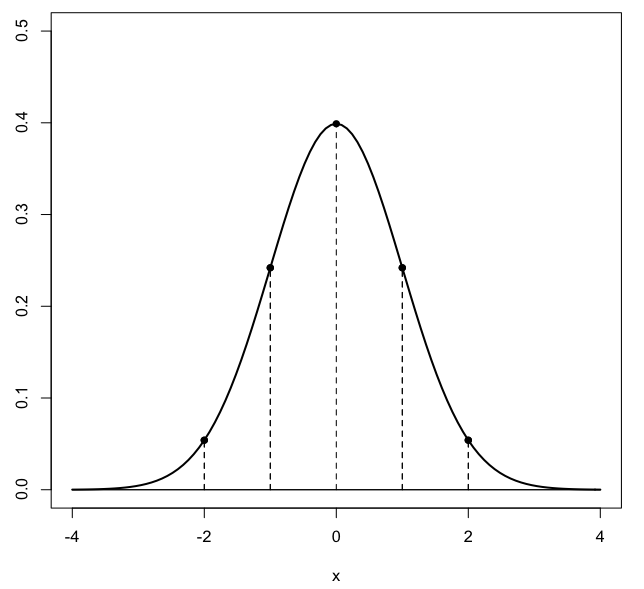
\includegraphics [scale=0.4] {gauss3.png} \end{center}
% \begin{bmatrix} a  &  b \\ c  &  d \end{bmatrix}
% \bigg |_

\large
\noindent
In this write-up I want to work with the spherical cap.  An example is shown in this figure from Wolfram
\begin{center} 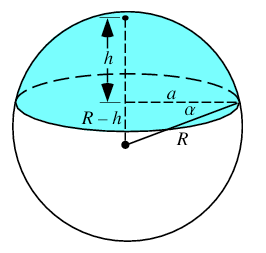
\includegraphics [scale=0.75] {spherical_cap.png} \end{center}

We have a sphere with radius $R$ and then a plane slicing through it, with a known height $h$ between the plane and the farthest point on the cap.  The radius of the circular base is $a$, where \[ a^2 = R^2 - (R-h)^2 \]
Here I will use a capital $H$ for the total height, so this becomes
\[ a^2 = R^2 - (R-H)^2 = 2RH - H^2 \]

Sometimes this figure is described as the part of a sphere which is inside a cylinder of radius $a$ and above the plane that gives a hemisphere.

What we would like to know is what are the volume and the surface area?

The volume can be done in various ways, some of them pretty easy.  For example, we originally derived the volume of the sphere (following Archimedes) as the sum of a series of horizontal slices, each of which is a circle of differing radius.  Then we add up all the slices.  We'll do that first.  It looks like this

\begin{center} 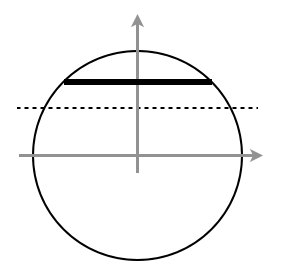
\includegraphics [scale=0.75] {spherical_cap2.png} \end{center}
The variable $h$ is the distance from the top of the sphere.  The value $H$ is the given height of the cap.  At each $h$ we have a circle with radius $a$ where 

\[ a^2 = 2Rh - h^2 \]
We compute the area of these circles, which is just

\[ A = \pi a^2 = \pi(2Rh - h^2)\]
Simply integrate this function for $h=0 \to H$

\[ V = \int A \ dh = \pi \int_0^H 2Rh - h^2 \ dh \]
\[ \pi(Rh^2 - \frac{1}{3}h^3) \ \bigg |_0^H \]
\begin{equation}
\boxed{V = \pi(RH^2 - \frac{1}{3}H^3)}
\end{equation}
Factor out as many $H$ as you like
\[ V = \pi(RH^2 - \frac{1}{3}H^3) = \pi H (RH - \frac{1}{3}H^2) = \pi H^2(R - \frac{1}{3}H) \]
This formula can also be written without $R$ by using the radius of the base $a$.  Start with one $H$ factored out
\[ V = \pi H (RH - \frac{1}{3}H^2) \]
\[ = \frac{1}{6} \pi H(6RH - 2H^2)  \]
Go back to $a^2$
\[ a^2 = 2RH - H^2 \]
\[ 3a^2 = 6RH - 3H^2 \]
\[ 3a^2 + H^2 = 6RH - 2H^2 \]
\begin{equation}
\boxed{ V = \frac{1}{6} \pi H(3a^2 + H^2)  }
\end{equation}

\subsection*{Shells}
\subsection*{Triple Integral}

to be continued

\subsection*{Surface area}



\end{document}  